\documentclass[10pt]{article}

% Packages
\usepackage[margin=1in]{geometry}   % 1 inch margins
\usepackage{fancyhdr}               % Custom headers/footers
\usepackage{lastpage}               % Reference total page number
\usepackage{graphicx}
\usepackage{caption}
\usepackage{comment}
\usepackage{subcaption}
\usepackage{titlesec}
\usepackage{array}
\usepackage[most]{tcolorbox}
\usepackage{cleveref}
\usepackage{pgfgantt}
\usepackage{adjustbox} % adjust the side of the gant chart
%%%%

%% Check to see which of the below are actually needed
\usepackage{amsmath}
\usepackage{graphicx}
\usepackage{geometry}
\usepackage{amsfonts}

\usepackage{tikz}
\usetikzlibrary{arrows.meta, positioning, shapes, fit}


\newcommand\Title{Fault Tolerant Quantum Repeaters}
% 


% Expanding and Developing....

\usepackage[numbers,sort]{natbib} % Cite things in order in the body
%% Removed from the data managemnt page
%\usepackage{times}
\usepackage{url}
\usepackage{color} % needed for todo
\usepackage{enumitem}
\usepackage{soul} % highlighting 
%\setlist{leftmargin=6.0mm, noitemsep}
\setlist{noitemsep}
\usepackage{cleveref} %Cref

\usepackage{xspace} % Needed for et al.
\newcommand{\ie}{\emph{i.e.,}\xspace}
\newcommand{\eg}{\emph{e.g.,}\xspace}
\newcommand{\etc}{etc.\xspace}
\newcommand{\etal}{\emph{et~al.}\xspace} 
%\newcommand{\acite}[1]{\citeauthor{#1}~\cite{#1}} % Not working

\newlist{learningObjectives}{enumerate}{1}
%\setlist[learningObjectives, 1]{leftmargin=.7in, label = LO\arabic*:, noitemsep}
%\setlist[learningObjectives, 1]{leftmargin=.13in, noitemsep}
\setlist[learningObjectives,1]{label={},noitemsep, leftmargin=.13in}% 
\newcommand{\LearningObjective}[3]{#1: #2 (#3)}
\newcommand{\descStep}[2]{\noindent \textbf{#1: } #2}
\newcommand{\smallTitle}[1]{\vspace{1mm} \noindent \textbf{#1: }}
\newcommand{\descIStep}[2]{\noindent \emph{#1: } #2} % Italics not just bold

\newcommand{\todo}[1]{\textcolor{cyan}{\textbf{[#1]}}}
\newcommand{\dan}[1]{\textcolor{blue}{{\it [Dan: #1]}}}
\newcommand{\travis}[1]{\textcolor{green}{{\it [Travis: #1]}}}
\newcommand{\jason}[1]{\textcolor{red}{{\it [Jason: #1]}}}




%\newcommand\Title{Contextual and Uncertainty-Aware Adaptive Quantum Error Management1}
\newcommand\MainTitle{Supporting Fault-Tolerant Quantum Repeaters with Contextual and Uncertainty-Aware Adaptive Quantum Error Management}

\setlist{noitemsep, leftmargin=6.0mm}

\usepackage{tikz}
\usetikzlibrary{shapes.geometric, arrows.meta, positioning}

% Header and footer setup
\pagestyle{fancy}
\fancyhf{} % Clear all header/footer fields

% Define values for the header

\fancyhead[L]{\MainTitle}
\fancyhead[C]{}
%\fancyhead[R]{dxkvse@rit.edu}
\fancyhead[R]{XXXXXX}


% Footer: Page x of y
\fancyfoot[C]{Page \thepage\ of \pageref{lastpage}}

% Title
\title{\vspace{-2cm} \bfseries \MainTitle}%: Integrating DRL, CMAB, and Post-Processing Strategies}
%\author{Daniel Krutz \{dxkvse@rit.edu\}\\}
\author{XXXX \{XXX@XXX.edu\}\\}

\date{}

%% Change the size of the section labels
\titleformat{\section}
  {\normalfont\bfseries\Large} % font and size %large
  {\thesection}{1em}{}              % section number formatting

%% Change the spacing between sections
\titlespacing*{\section}
  {0pt}   % Left margin
  {1ex}   % Space before the section
  {0.5ex} % Space after the section

\begin{document}

%% start defining the layout of the 1st page
\fancypagestyle{firstpage}{
  \fancyhf{}              % Clear all header/footer
  \renewcommand{\headrulewidth}{0pt} % No header rule
  \fancyfoot[C]{Page \thepage\ of \pageref{lastpage}} 
}
%% end defining the layout of the 1st page

\maketitle
%\thispagestyle{fancy} % Apply fancy header/footer to title page
%\thispagestyle{empty} % Suppress header/footer on the first page
\thispagestyle{firstpage}

\vspace{-8mm}
{\par\centering
 \begin{tcolorbox}[enhanced, width=1.03\linewidth, 
            %colback=blue!50!white!20,
            arc=0pt, outer arc=0pt, 
            borderline={1.5pt}{0pt}{black!90},
            borderline={0.25pt}{3pt}{black!70, sharp corners},
            drop fuzzy shadow]
    \centering
{\large %\textbf{Synopsis}
\par\medskip}
\normalsize%\itshape
Intelligently apply real-time/post processing error management strategies to Fault Tolerant Quantum Repeaters (FTQR) to enable effective, but resource friendly error management.
\end{tcolorbox}\par}

%%%%%%%%%%%%%%%%%%%%%%%%%%%%%%%%%%%%%%%%%%%%%%%%%%%%%%%




%%%%%%%%%%%%%%%%%%%%%%%%%%%%%%%%%%%%%%%%%%%%%%%%%%%%%%%%
%%%%%%%%%%%%%%%%%%%%%%%%%%%%%%%%%%%%%%%%%%%%%%%%%%%%%%%%
%%%%%%%%%%%%%%%%%%%%%%%%%%%%%%%%%%%%%%%%%%%%%%%%%%%%%%%%



\begin{figure}[h!]
\centering
\scalebox{0.99}{
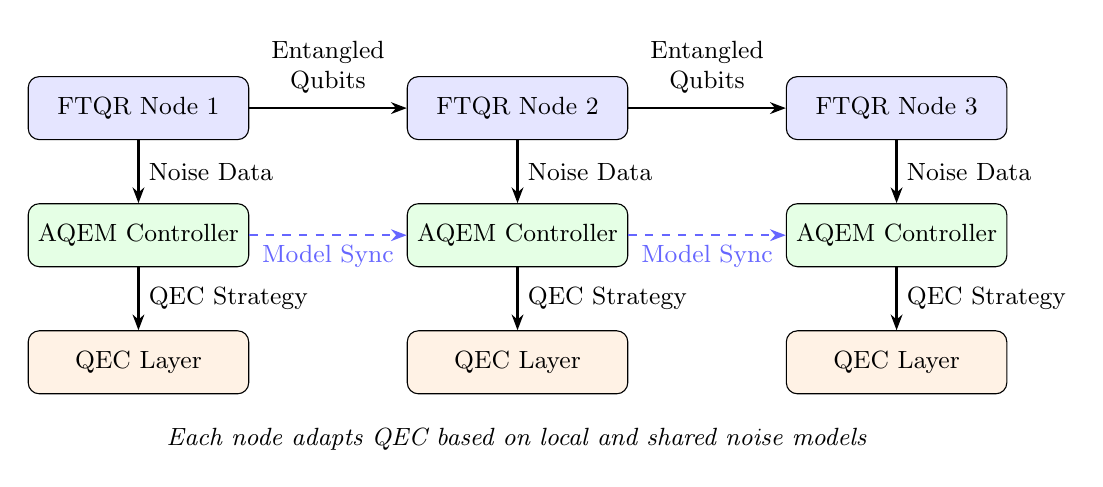
\begin{tikzpicture}[
  node distance=0.8cm and 2cm,
  box/.style={rectangle, draw, rounded corners=4pt, minimum width=2.8cm, minimum height=0.8cm, align=center},
  arrow/.style={-{Stealth[length=2mm]}, thick},
  dashedbox/.style={rectangle, dashed, draw, rounded corners=6pt, inner sep=5pt, fill=blue!2},
  every node/.style={font=\small}
]

% Nodes for Repeaters
\node[box, fill=blue!10] (R1) {FTQR Node 1};
\node[box, fill=blue!10, right=of R1] (R2) {FTQR Node 2};
\node[box, fill=blue!10, right=of R2] (R3) {FTQR Node 3};

% AQEM controllers below each
\node[box, fill=green!10, below=of R1] (A1) {AQEM Controller};
\node[box, fill=green!10, below=of R2] (A2) {AQEM Controller};
\node[box, fill=green!10, below=of R3] (A3) {AQEM Controller};

% QEC layer below AQEM
\node[box, fill=orange!10, below=of A1] (Q1) {QEC Layer};
\node[box, fill=orange!10, below=of A2] (Q2) {QEC Layer};
\node[box, fill=orange!10, below=of A3] (Q3) {QEC Layer};

% Communication arrows (Quantum channel)
\draw[arrow] (R1) -- node[above]{\begin{tabular}{c}Entangled\\Qubits\end{tabular}} (R2);
\draw[arrow] (R2) -- node[above]{\begin{tabular}{c}Entangled\\Qubits\end{tabular}} (R3);


% Vertical connections (AQEM + QEC)
\foreach \x/\y in {R1/A1, R2/A2, R3/A3} {
  \draw[arrow] (\x) -- node[right]{Noise Data} (\y);
}
\foreach \x/\y in {A1/Q1, A2/Q2, A3/Q3} {
  \draw[arrow] (\x) -- node[right]{QEC Strategy} (\y);
}

% Distributed learning connections between AQEMs
\draw[arrow, dashed, blue!60] (A1) -- node[below]{Model Sync} (A2);
\draw[arrow, dashed, blue!60] (A2) -- node[below]{Model Sync} (A3);

% Labels
\node[below=0.3cm of Q2] {\textit{Each node adapts QEC based on local and shared noise models}};

\end{tikzpicture}
}
\caption{XXXXXX.}
\label{fig:AQEMarchitecture}
\end{figure}


%%%%%%%%%%%%%%%%%%%%%%%%%%%%%%%%%%%%%%%%%%%%%%%%%%%%%%%%
%%%%%%%%%%%%%%%%%%%%%%%%%%%%%%%%%%%%%%%%%%%%%%%%%%%%%%%%
%%%%%%%%%%%%%%%%%%%%%%%%%%%%%%%%%%%%%%%%%%%%%%%%%%%%%%%%





% Later on down the road, focus on multi agent learning













\dan{proofread all}
\dan{If sendint to the DOE, make sure to tie into any specific calls that they have}

\section*{Overview}
Fault-tolerant quantum repeaters (FTQR) provide error-corrected, high-fidelity transmission of quantum information across long distances by continuously detecting and correcting errors during entanglement and communication processes. FTQR represent the future of quantum data networking. FTQR utilize various QEC strategies to ensure that data is correct. In traditional quantum repeaters, error correction strategies remain static and preconfigured, failing to account for temporal and spatial variations in hardware noise, photon loss, and entanglement fidelity. The current implementation of FTQR are limited by several factors including very high resource requirements, quantum memory and coherence limitations, complexity of error correction at the network scale.


The objective of this work is to support the more efficient implementation of FTQR through a more efficient and effective implementation of QEC strategies. This will be addressed through the development, implementation and evaluation of the `Adaptive Quantum Error Mitigation' (FTQR-AQEM) framework. This framework will provide dynamic, context-aware error management for fault-tolerant quantum repeaters, improving end-to-end entanglement fidelity while efficiently allocating limited qubit and computational resources. By integrating predictive modeling, adaptive QEC selection, and decentralized decision-making, it enables robust, scalable, and resource-efficient quantum communication across noisy and variable network conditions.

% What are some current inherint limitations of FTQR and how will the proposed work address these






%This will be accomplished by implementing our ?lightweight? AQEM framework to support FTQR in implementing the most effective QECC in the most efficent manner possible.






\subsection*{Framework Overview}

Our proposed `Fault-Tolerant Quantum Repeater Adaptive Quantum Error Management' (FTQR-AQEM) framework will provide an intelligent, self-optimizing approach for maintaining the fidelity and stability of entangled quantum states across long-distance quantum communication networks. Traditional quantum repeaters enable quantum information transmission by performing entanglement swapping and purification at intermediate ?repeater? nodes. However, these systems remain highly sensitive to accumulated noise, decoherence, and operational imperfections. As technology progresses, quantum data networks (QDNs) are expected to be ``fault tolerant'' in that they are able to detect, correct, and adapt to quantum errors in real time, maintaining high-fidelity entanglement and reliable information transfer even in the presence of noise, decoherence, and hardware imperfections. FTQR are difficult to currently realize due to the large amount of resources that they require.

The FTQR-AQEM framework will support the implementation of FTQR and addressing particular resource challenges by embedding a real-time adaptive control layer that dynamically selects and tunes quantum error correction (QEC) strategies according to observed and predicted noise profiles.

Formally, the fidelity of an entangled state transmitted through a sequence of $N$ repeater nodes can be expressed as:
\begin{equation}
F = \prod_{i=1}^{N} (1 - \epsilon_i),
\end{equation}
where $\epsilon_i$ represents the effective error rate at repeater $i$. Without fault tolerance, $\epsilon_i$ accumulates rapidly, degrading $F$ below operational thresholds. The FTQR-AQEM framework mitigates this by incorporating a predictive noise estimation process and adaptive QEC selection mechanism, minimizing $\epsilon_i$ in real time. This results in a self-regulating repeater chain capable of maintaining $F \geq F_{\text{thresh}}$, where $F_{\text{thresh}}$ is the fidelity threshold for fault-tolerant entanglement distribution.

The adaptive component of AQEM employs a Bayesian learning process to predict the noise variance $\sigma_t^2$ at each repeater node based on both historical and contextual quantum channel information:
\begin{equation}
P(\sigma_t^2 | \mathcal{D}_t) \propto P(\mathcal{D}_t | \sigma_t^2) P(\sigma_t^2),
\end{equation}
where $\mathcal{D}_t$ denotes the set of measurement data and syndrome outcomes up to time $t$. Using this predictive posterior, the framework selects the optimal QEC code $C^*$ from a candidate set $\{C_1, C_2, \dots, C_k\}$ that minimizes expected logical error rate:
\begin{equation}
C^* = \arg\min_{C_i} \mathbb{E}[\epsilon_{\text{logical}}(C_i | \sigma_t^2)].
\end{equation}
This enables each repeater to autonomously balance QEC overhead and error mitigation performance, adapting to time-varying conditions such as qubit loss, gate noise, or environmental drift.



%% Remove this part
From a distributed systems perspective, FTQR-AQEM forms a scalable quantum data network by enabling repeaters to share compressed error statistics, fidelity metrics, and predicted noise models. Each repeater operates as a semi-autonomous agent within a cooperative network, updating shared parameters through limited quantum-classical feedback. This distributed learning approach allows the network to collectively adapt to global changes, such as channel degradation or varying entanglement demands, without requiring centralized control.


\subsection*{Distributed/Scalable Component}
Each of the FTQR will contain a local AQEM agent to support the individual agent's decision-making process. This agent will monitor its own qubits, error syndromes, and channel telemetry. Each of the FTQR-AQEM agents can share a compressed context summaries (\eg estimated noise levels, uncertainty bounds, link quality metrics) with adjacent nodes. This decentralized exchange of information can support decentralized coordinated adaptation. The use of federated reinforcement learning or hierarchical self-organizing maps (GHSOM) will enable each FTQR agent to learn locally, while contributing to the greater optimization of all FTQR agents.



\subsubsection*{Addressed Challenges in FTQR}

\begin{itemize}
    \item Non-adaptive error management
    \begin{itemize}
        \item \textbf{Limitation:} Traditional repeaters use static QEC strategies that cannot respond to varying noise or channel conditions.
        \item \textbf{FTQR-AQEM Solution:} Dynamically selects QEC and post-processing strategies based on real-time telemetry and predictive modeling to maintain high fidelity under changing conditions.
    \end{itemize}

    \item Inefficient resource utilization
    \begin{itemize}
        \item \descStep{Limitation}{Static QEC often overuses physical qubits or applies full error correction unnecessarily, wasting ancilla and computation resources.}
        \item \descStep{FTQR-AQEM Solution}{Employs resource-aware policies that balance logical fidelity with qubit overhead, only applying costly correction when it maximizes utility.}
    \end{itemize}

    \item Vulnerability to non-stationary noise
    \begin{itemize}
        \item \descStep{Limitation}{Environmental drift, channel loss, and temporal variations in hardware degrade entanglement reliability.}
        \item \descStep{FTQR-AQEM Solution}{Uses hierarchical context modeling and predictive uncertainty estimates to anticipate noise fluctuations and adapt QEC parameters proactively.}
    \end{itemize}

    \item Limited scalability of decision-making
    \begin{itemize}
        \item \descStep{Limitation}{As networks grow, manually configured or static QEC policies cannot scale efficiently across multiple repeaters.}
        \item \descStep{FTQR-AQEM Solution}{Implements decentralized, multi-agent adaptive control where each repeater autonomously optimizes QEC while coordinating minimal context with neighbors.}
    \end{itemize}

    \item Suboptimal entanglement fidelity under probabilistic link generation
    \begin{itemize}
        \item \descStep{Limitation}{Randomized entanglement swapping and photon loss can produce logical errors that static strategies fail to correct efficiently.}
        \item \descStep{FTQR-AQEM Solution}{Integrates real-time feedback and reinforcement learning to select corrective actions like re-encoding or purification only when needed, improving end-to-end fidelity.}
    \end{itemize}

    \item Inability to balance fidelity and operational latency
    \begin{itemize}
        \item \descStep{Limitation}{High-fidelity QEC can introduce delays, reducing effective network throughput.}
        \item \descStep{FTQR-AQEM Solution}{Optimizes QEC and post-processing decisions to maximize fidelity per unit time, trading off correction intensity against latency in a context-aware manner.}
    \end{itemize}
\end{itemize}


% Proofread all of this




\section*{Related Works}
% If nothing else, have this section so that we can directly compare our work against theirs



\subsection*{Risks and Limitations}


% FTQR are still very resource-intensive. How would this be addressed, even with AQEM

% 



\label{lastpage}
%\cleardoublepage


%\appendix


%% DK: Put onto a different page since it does not count against the page limit
%\setcounter{page}{1}

%\cfoot{\thepage}
%\pagenumbering{roman}
%\section{Appendix}

%\input{sections/Appendix.tex}


%% I think the appendix goes before the bib. Otherwise, I could see people missing it
%\newpage
%\pagebreak
%\addcontentsline{toc}{section}{References}
%\bibliographystyle{plain}
%\bibliography{refs}
\end{document}



